%%%%%%%%%%%%%%%%%% DOCUMENT SETUP %%%%%%%%%%%%%%%%%%

% Required IEEE parameters
\documentclass[letterpaper, 10pt, conference]{IEEEtran} % set document type
\IEEEoverridecommandlockouts                              % for \thanks command
%\overrideIEEEmargins                                      % use for \addtolength to normalize column lengths


% Packages
\usepackage{graphicx} % allows additional graphics formats
  \graphicspath{ {./images/} }
\usepackage{amsmath}   % assumes amsmath package installed
  \allowdisplaybreaks[1] % allow eqnarrays to break across pages
  

\usepackage{amssymb}   % assumes amsmath package installed 
\usepackage{url}       % format hyperlinks correctly
\usepackage{rotating}  % allow portrait figures and tables
\usepackage{subfigure} % allow matrices of figures
\usepackage{float}     % allows H option on floats to force here placement
\usepackage{multirow}  % allows merging of rows in tables
\usepackage{tabularx}  % allows fixed width tables
\usepackage{siunitx}
\usepackage{placeins}
\usepackage[ruled,vlined]{algorithm2e}
\include{pythonlisting}
\usepackage{tikz}
\usetikzlibrary{positioning,angles,quotes,automata}

\usepackage{ctable}    % modifies \hline for use in table
\usepackage{bm}        % allow bold fonts in equations
\usepackage{wrapfig}   % allow text wrapping round figures
\usepackage{stfloats}  % control placement of floats
\usepackage[backend=biber,style=ieee,maxbibnames=3,bibencoding=utf8]{biblatex}   % allow bibliography control 
	
    \addbibresource{journal_abbreviations.bib }
\addbibresource{references.bib}
\usepackage{siunitx}
\usepackage{placeins}

% Custom commands

\newcommand{\rvs}{r.v.'s\xspace}
\newcommand{\mdp}{Markov Decision Process\xspace}
\newcommand{\mdps}{Markov Decision Processes\xspace}
\newcommand{\mrp}{Markov Reward Process\xspace}
\newcommand{\mc}{Markov Chain\xspace}

\def\given{\;\middle\vert\;}
\def\optimal{\star}
\def\transpose{\intercal}
\def\laplacian{\mathbf{\mathcal{L}}}
\def\eqdef{\overset{\underset{\mathrm{def}}{}}{=}}
\def\indicator{\mathds{1}}
\DeclareMathOperator{\expectation}{\mathbb{E}}
\DeclareMathOperator{\vol}{\text{vol}}

\newcommand{\todo}[1]{[TODO: #1]}
\newcommand{\termidx}[1]{\index{#1}{\textbf{#1}}}

\usepackage{amsmath}


\newcommand{\matlab}{\emph{\sc{Matlab}}}
\newcommand{\maple}{\emph{\sc{Maple}}}
\newcommand{\simulink}{\emph{\sc{Simulink}}}
\newcommand{\dc}{d.c.}
\newcommand{\ac}{a.c.}
\newcommand{\rms}{RMS}
\newcommand{\wgn}{{\tt wgn}}
\newcommand{\sus}[1]{$^{\mbox{\scriptsize #1}}$}
\newcommand{\sub}[1]{$_{\mbox{\scriptsize #1}}$}
\newcommand{\chap}[1]{Chapter~\ref{#1}}
\newcommand{\sect}[1]{Section~\ref{#1}}
\newcommand{\fig}[1]{Fig.~\ref{#1}}
\newcommand{\tab}[1]{Table~\ref{#1}}
\newcommand{\equ}[1]{(\ref{#1})}
\newcommand{\appx}[1]{Appendix~\ref{#1}}
\newcommand{\degree}{\ensuremath{^\circ}}
\newcommand{\Vrms}{V\sub{\rms}}
\newcommand{\Vpp}{V\sub{pp}}
\newcommand{\otoprule}{\midrule[\heavyrulewidth]}         
\newcolumntype{Z}{>{\centering\arraybackslash}X}  % tabularx centered columns 
\usepackage{comment}

% Adjust figure spacing to get more text onto each page
\setlength{\abovecaptionskip}{2pt}
\setlength{\belowcaptionskip}{2pt}
\setlength{\dbltextfloatsep}{8pt}
\setlength{\dblfloatsep}{3pt}
\setlength{\floatsep}{3pt}
\setlength{\textfloatsep}{2pt}
%\addtolength{\skip\footins}{-10pt}
% http://www.jmlr.org/papers/volume17/15-252/15-252.pdf

%%%%%%%%%%%%%%%%%% TITLE AND FRONT MATTER %%%%%%%%%%%%%%%%%%

% Title
\title{\LARGE \bf Markov Chain Decision Process for Adaptive Transmission Policy in Wearable Sensors }

% Authors and affiliations 
\author{Tahmina Zebin, Niels Peek and Alexander~J.~Casson,~\IEEEmembership{Senior Member,~IEEE}%
\thanks{This work was supported by the UK Engineering and Physical Sciences Research Council grant number EP/P010148/1.}%
\thanks{T. Zebin and A. J. Casson are with the School of Electrical and Electronic Engineering, The University of Manchester, Manchester, UK. Email: \tt{\small{\{tahmina.zebin,alex.casson\}@manchester.ac.uk}}.}%
\thanks{ N. Peek is with the Health e-Research Centre, The University of Manchester, Manchester, UK. Email: \tt{\small{\{niels.peek\}@manchester.ac.uk}}.}%
}%

% Setup document 
\begin{document}
\maketitle
\thispagestyle{empty} % stop page numbers
\pagestyle{empty}

%%%%%%%%%%%%%%%%%% ABSTRACT



%%%%%%%%%%%%%%%%%%
\begin{abstract}
Designing systems that responds to user’s context or change of context only is a current research need instead of continuous monitoring with wearable sensors  due to limited battery capacity in such systems. The usage of the battery can be reduced if the sensor setting is adapted to each context. 

One of the solutions, consumed less energy than the single setting policy, while sacrificing very little in terms of accuracy.

\end{abstract}
%%%%%%%%%%%%%%%%%% INTRODUCTION %%%%%%%%%%%%%%%%%%
\section{INTRODUCTION}

\label{sec:introduction}
% The availability and spread of wearable sensing devices has made them suitable to use in non-invasive monitoring of the user's behavior patterns, to check on their health and activities, and finally providing them person-specific recommendations.
The wearable sensing systems generate raw data that is processed into knowledge by reasoning and machine learning algorithms \cite{Xenofon2017}. Continuous sensing and data processing requires the wearable sensing module to constantly run at full power, thereby rapidly depleting the system’s energy, which is a critically
constrained resource \cite{krause2005}. As energy consumption is a major concern in context-aware wearable sensing \cite{Yan2012}, the main objective of this paper is to efficiently find an assignment of settings to contexts that generates good trade-offs between system energy consumption and system quality (for example: accuracy of the context recognition).



To reduce energy consumption and increase the
deployment lifetime of the wearable sensor, we utilize the fact that, human activity is a rather continuous process: observed at a particular point in time, a person involved in one activity is likely to continue the activity than to change to another. We exploit this continuity by proposing a selective sampling strategy. 

The simplest energy saving algorithm would be the one that infuses into the low-level sensory operations by changing the sampling intervals.
Although sensor duty cycling might be applied to reduce energy consumption, there exist two major problems that need to be carefully investigated:
(1) how to accurately estimate the underlying state when
the sensor stays idle? and 
(2) given an energy budget, how should sensor sampling be scheduled intelligently such that the expected state estimation error can be minimized?



We propose an adaptive sensing mechanism that dynamically assigns duty cycles (DCs) and sampling periods in a context-aware manner would reduce power consumption significantly. However, intervening sensory operations to achieve power efficiency reduces the accuracy, i.e., quality of service, provided by context-aware services. Therefore, it creates a trade off between power consumption and accuracy provided by the system.

The analytical modeling of the accelerometer sensor is provided and integrated into the sensing mode scheduler. The system aims at utilizing a mixture pair of duty cycling and adaptive sampling regulated by a few suboptimal sampling policies to prolong mobile device battery lifetime.



We propose a Markov decision process (MDP) method that efficiently finds near-optimal sensor settings for each context. While standard MDP is aimed solely at maximizing expected future rewards (value), the circular flow of performance matrices between the agent and its environment is generally ignored. In particular, the information gained from the environment by means of perception and the change involved in the process of action selection (i.e., control) are not treated in the standard MDP setting \cite{Rubin2012}. In this paper, we focus on the accuracy and energy consumption information in the learning mechanism and show how it can be combined with the reward measure in a unified way. Both of these measures satisfy the familiar Bellman recursive equations \cite{bellman2015} , and their linear combination (the free-energy) provides an interesting new optimization criterion. 
In basic terms, the Reinforcement Learning (RL) is the problem in an area of machine learning concerned with how a learning agent learns what to do (action) in a given situation (state) by interacting with an environment to maximize or minimize numerical returns (rewards).
The Markov chain model simulates the behavior of the system in different configurations and a multi-objective algorithm finds a set of configurations that fulfills the required system quality requirement. The method was evaluated on an in-house daily-life activity dataset and found good trade-offs between the system’s energy expenditure and the system’s accuracy. The accuracy of the models are based on the effectiveness of the algorithms

 Our results indicate that optimized sampling schemes can increase
the deployment lifetime of a wearable computing platform by a factor of four without a significant loss in prediction accuracy. 



%%%%%%%%%%%%%%%%%% BACKGROUND %%%%%%%%%%%%%%%%%%
\section{Related Work}
The recognition of human context has received a significant attention in the medical field, because it is a task of interest for many applications, including assisted living of elderlies, physical assessment, and supervision of patient with chronic diseases such as serious mental illness, dementia, obesity.  In a typical scenario, wearable sensors like accelerometers or ECG are attached to the patient to measure biomechanical, physiological and environmental data \cite{RAULT201723}.

Satisfactory trade-off between three optimization criteria: low energy consumption, high recognition accuracy and low latency.  

\subsection{Energy-efficient systems}
Continuous sampling and communication tasks quickly deplete sensors’ battery, and frequent charging may  not be convenient for day to day monitoring \cite{Rault2017}. Therefore, there is a need to develop energy-efficient solutions for long-term monitoring applications in order to foster the acceptance of these technologies.

Lifetime maximization can be by having power-on time reduction, communication reduction, computation reduction strategies.Ideally,  a designer will need to apply strategies from all
these categories to maximize the lifetime of the human context recognition appplication.

\begin{itemize}
\item Energy efficient Mechanism for lifetime maximization
\item{Power-on time reduction}
\begin{itemize}
    \item  Deactivate Power hungry sensors\cite{rahmati2007context,Nath2013,Park2011}
    To achieve a good trade-off between the number of sensors activated and the classification accuracy. Indeed, the usage of many sensors may increase the recognition accuracy at the expense of additional energy consumption.
    
    \item{Context based pull services\cite{Rachuri2011,paschou2013health}}
    
\end{itemize}
\item Communication Reduction
\begin{itemize}
    \item Adaptive sampling rate\cite{qi2013adasense,Yan2012}. 
    Maurer et al. \cite{maurer2006activity} studied the impact of the accelerometer sampling rate on the recognition accuracy and they found that no significant gain in accuracy is achieved above 20 Hz for ambulation activities. Therefore, depending on the user activity and the type of sensor, it may not be necessary to sample at the maximum rate in order to achieve a desired accuracy. The key idea behind adaptive sampling rate is to adapt the frequency of data acquisition depending on the recognized context. This technique leads to fewer samples, which will result in less data to transmit.
    \cite{yan2012energy} propose to adapt both the sampling rate (SR) and the classification feature (CF) in real-time. For each activity they compute offline the accuracy that can be achieved for different tuple ⟨SR, CF⟩ of sampling rate and classifier feature. Then, depending on the strategy, they determine per activity the optimal tuple that can achieve a user-specified accuracy, or the tuple that has the highest ratio of accuracy over energy consumption. At runtime, when an activity is recognized, the application selects the corresponding tuple
⟨SR, CF⟩ which enables to tradeoff energy and accuracy. Qi et al.\cite{qi2013adasense} introduced the idea that it requires
a lower sampling rate to determine whether a specific activity happens or not than classifying multiple activities. The architecture decides whether the current activity changes or not through single activity event
detection with a lower sampling rate. If a change is detected, AdaSense switches to the multi-activity classification at a
higher sampling rate. Then the solution performs event detection of the new activity at a lower sampling rate. The major
drawback of these solutions is the lack of flexibility as configurations are selected once and for all for a given activity, which
requires a new training phase when considering new activities.
    
    \item  On-board Computation\cite{chu2011balancing}
\end{itemize}
\item  Computation Reduction
\begin{itemize}
    \item Adaptive classifier operations\cite{wang2013energy}
    \item  Feature subset selection\cite{chu2011balancing}
    There exists a trade-off between delay and accuracy since using a lot of features certainly
enhances the accuracy but it is energy and computation consuming. Inversely, reducing the number of features allows saving
energy and reducing computation at the cost of reduced accuracy. Pareto-based Multiobjective Optimization reported in \cite{cilla2009creating} that selects feature subsets whose size is minimized
while maximizing the accuracy of the classifier. Their approach provides the designer with diversified solutions closed to
the Pareto-front. The advantage is that the expert does not have to set a priori tradeoff between accuracy and number of
feature and select a subset that best fits the application requirement knowing that these solutions are
close to the optimal. In \cite{qi2013adasense}, a genetic programming based algorithm is used to explore the feature set, with the objective to
minimize the sampling rate while achieving a given accuracy.
    
    \item Opportunistic resource sharing\cite{cilla2009creating}.
\end{itemize}
\item  Markov Decision Processes used in body sensor Networks
\begin{itemize}
    \item \cite{Alsheikh2015MDP,au2011carer,zois2013unified,pietrabissa2013optimal}
    
\end{itemize}
 
\end{itemize}


\subsection{Motivation}

Most of the system focused on sensed data instead of information.  The sampling frequency cannot be controlled directly and are not sensitive of information. We need satisfactory trade-off between three optimization criteria: low energy consumption, high recognition accuracy and low latency.



To design smart wearable sensors that are capable of capturing and evaluating raw sensor data to infer actions, activities or behaviors \cite{Yurur2015}, is becoming a well-established research domain, particularly within the realm of human activity recognition (HAR) and location-based services. Most studies reported in the literature rely on recognition of user activities and recognizing common daily life activities and  behaviors by proposing and implementing various machine learning models. 



State-based systems with discrete or continuous time are often modelled with the help of Markov chains. In order to specify performance measures for such systems, one can define a reward structure over the Markov chain, leading to the Markov Reward Model (MRM). Typical examples of performance measures that can be defined in this way are time-based measures (e.g. mean time to failure), average energy consumption, monetary cost (e.g. for repair, maintenance) or even combinations of such measures. These measures can also be regarded as target objectives for system optimization. For that reason, an MRM can be enhanced with an additional control structure, leading to Markov Decision Processes (MDP) \cite{Gouberman2014}.

MDPs for reasoning about the actions of an autonomous decision-making agent in an wearable sensing system  will aim to achieve long-term objective of saving battery life while maintaining reasonable accuracy for detecting a certain activity.

Human action selection is driven by multiple
competing objectives; for example, a medical decision will be based not only on the effectiveness
of a treatment, but also on its potential side-effects, cost, and other considerations.Because the relative importance of these objectives varies from user to user, the quality of a policy is not well captured by a universal single scalar “reward” or “value.” Multi-Objective
Markov Decision Processes (MOMDPs) accommodate this.
 
 \begin{figure}
    \centering
    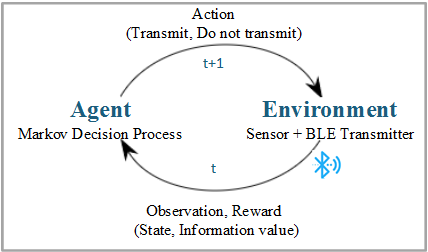
\includegraphics[width=0.35\textwidth]{images/RL.png}
    \caption{Reinforcement learning Scenario for the wearable sensor data transmission}
%     \label{fig:f1_score}
  \end{figure}
  \begin{figure*}
    \centering
      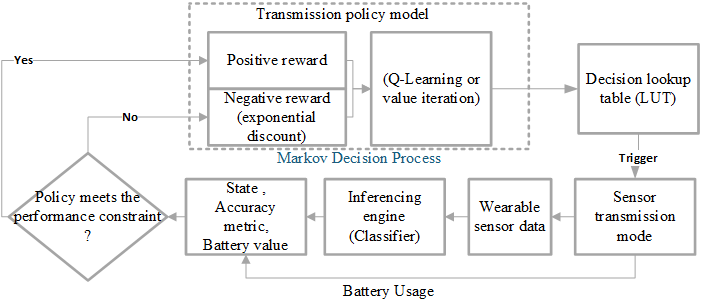
\includegraphics[width=0.69\textwidth]{images/MDP3.png}
\caption{Execution of the decision process}
    \label{fig:confusion}
  \end{figure*}
  
%  \begin{figure*}
%    \centering
%      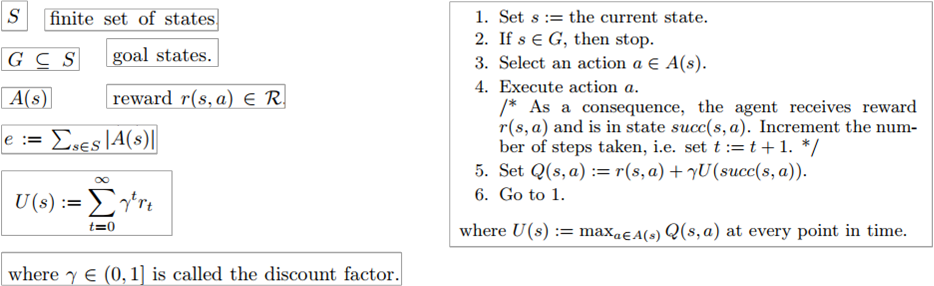
\includegraphics[width=0.69\textwidth]{images/algorithm.png}
%\caption{Q-learning algorithm for optimal policy selection}
%    \label{fig:confusion}
%  \end{figure*}

  \begin{figure*}
    \centering
    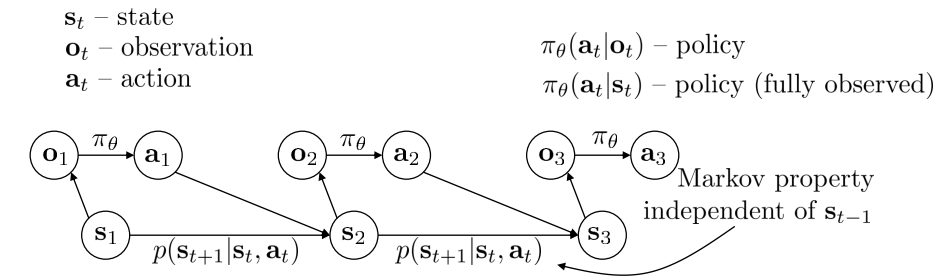
\includegraphics[width=0.79\textwidth]{images/Policy.PNG}
\caption{Observation contains monitoring of multiple objectives}
    \label{fig:markov}
  \end{figure*}
 \begin{figure}
    \centering
    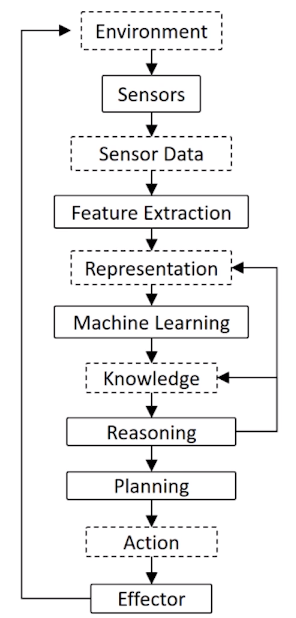
\includegraphics[width=0.25\textwidth]{images/reiforcement_learning.png}
\caption{}
    \label{fig:markov}
  \end{figure} 


The objective f

\section{Markov Decision Process} 
\subsection{Definition}
Major components of an RL Agent are Policy, Value Function and Model. A state $S_t$ is Markov if and only if
\begin{equation}
\mathbb{P}[S_{t+1}|S_t] = \mathbb{P}[S_{t+1}|S_1, ... , S_t]
\end{equation}
A future is independent of the past given the present. We use state transition matrix $P$ to define transition probabilities from all states $s$ to all successor states $s'$
\begin{equation}
P_{ss'}=\mathbb{P}[S_{t+1}=s'|S_t=s]
\end{equation}
A Markov Reward Process is a tuple $<S, A, P, R, \gamma>$
\begin{itemize}
	\item $S$ is a finite set of states
	\item $A$ is a finite set of actions
	\item $P$ is a state transition probability matrix,
		  $$P_{ss'}^{a} = \mathbb{P}[S_{t+1} = s'| S_t = s, A_t = a]$$
	\item R is a reward function, $$R_s^a = \mathbb{E}[R_{t+1}|S_t=s, A_t = a]$$
	\item $\gamma$ is a discount factor, $\gamma \in  [0, 1]$


\item Return $G_t$ $$G_t=\sum_{k=0}^{\infty} \gamma^k R_{t+k+1}$$

\item State value function $v_\pi (s)$
$$v_\pi (s) = \mathbb{E}_\pi [G_t|S_t = s]$$
\item Action value function $q_\pi (s, a)$
$$q_\pi (s, a) = \mathbb{E}_\pi [G_t|S_t = s, A_t = a]$$
\item Policy $\pi$ $$\pi (a|s) = \mathbb{P}[A_t = a|S_t=s]$$
\end{itemize}

\subsection{Planning by Dynamic Programming}


  
  


% \begin{tikzpicture}[auto,node distance=8mm,>=latex,font=\small]
%     \tikzstyle{round}=[thick,draw=black,circle]

%     \node[round] (s0) {$s_0$};
%     \node[round,above right=0mm and 20mm of s0] (s1) {$s_1$};
%     \node[round,below right=0mm and 20mm of s0] (s2) {$s_2$};

%     \draw[->] (s0) -- (s1);
%     % Adding invisible marker node below with "node [very near start, anchor=center] (m1) {}"
%     \draw[->] (s0) -- node [very near start, anchor=center] (m1) {} (s2);
%     % Here too, with "node [very near start, anchor=center] (m2) {}"
%     \draw[->] (s0) [out=40,in=100,loop] to node [very near start, anchor=center] (m2) {} (s0);
%     % Now, this new path draws directly between our two markers. 
%     % Tweak the angle depending on the situation.
%     \draw (m1.center) edge [bend right=50] (m2.center);
% \end{tikzpicture}


\section{Q-Learning}
Q-learning is an online algorithm that performs reinforcement learning. The algorithm calculates the quality of a state-action pair which is denoted by Q and is initialized to zero at the beginning of the learning phase. At each step of environment interaction, the agent observes the environment and decides on an action to change state based on the current state of the system. The algorithm calculates the quality of a state-action pair which is denoted by Q and is initialized to zero at the beginning of the learning phase. At each step of environment interaction, the agent observes the environment and decides on an action to change state based on the current state of the system. 

 The agent keeps a value function $Q^{π} (s(t), a(t))$ according to an action performed which maximizes the long-term rewards. The Q-factor update equation with discounted reward is as follows: 
%begin{equation}
 %     Q^{t+1}(s(t + 1), a(t)) = Q^{t}(s(t), a(t)) + {\alpha}(s(t), a(t))[R(t)  +\\
 % {\gamma} MAX Q^{t}(s(t+1), a(t))- Q^{t}(s(t), a(t))]
%\end{equation}





    
  \subsection{Problem description}
  Suppose we have a wearable sensor that works as follows:
 The user is in one of the predefined contextual states $s \in S$ and
each context is associated with some action setting $a\in A$.

 Settings can be  whether to have the sensor in active(transmit) or sleep (do not transmit) mode , which sensors to use( i.e. accelerometer only or gyroscope), or what sampling
frequency to use( e.g. 50 Hz or 10Hz) and so on.
A setting is used as long as the system believes that user is in a context that corresponds to that setting. When a context
change is detected by the system, the setting is changed
accordingly. For example, if we are sitting we might use a
low sensor sampling frequency, but when walking is detected,
a higher sampling frequency can be turned on.
The most straightforward way to determine the optimal assignment of settings to contexts for such a system is to
simply try out every assignment. This approach has two
obvious problems that make it infeasible for a large number
of settings and/or contexts. 
To evaluate one of the assignments; appropriate
machine learning models should be created  and then run through all the
data in the dataset, classifying instances while simulating
different settings and switching between them accordingly. This process can be prohibitively slow (lasting seconds or
minutes).

In this work, we considered a scheme where each context is assigned a setting. Those settings then change as different contexts are recognized. However, by adapting a Markov chain model, similar system schemes can be constructed and evaluated. 



    
    \subsection{Dataset Preparation}
To reduce energy consumption and increase the
deployment lifetime of the wearable sensor, we utilize the fact that, human activity is a rather continuous process: observed at a particular point in time, a person involved in one activity will be more likely to continue the activity than to change to another. We exploit this continuity by proposing an adaptive sampling strategy.

The adaptive sampling method reduces
the number of observations to save energy, from a continuous monitoring to selected time points, while keeping the accuracy of tracking the user’s current activity as high as possible.


 \section{MDP formulation } 
 
We can model the adaptive sampling problem as a sequential decision-making process, where we decide at each time step whether we want to sample and use the classifier to estimate the user’s activity.

System state, $s_{t}={Activity Label, Probabilistic Decision Value, Energy Available}$.
Action Space, $a_{t}={0=no transmission, 1= transmission mode 1, 2= transmission mode 2}$.

If $\rho_1$ is the probabilistic decision value in transmission mode 1, and a change of activity label is detected, we use a reward function

The next state of the system depends only on the current state and action taken

A conditional plan $\pi$ is a sequence of decisions, which, depending on the outcome of the observations made so far, decides when the next observation should be made.  For each activity
sequence $\boldsymbol{a}$, the selected observation times are denoted
by $\pi(\boldsymbol{a})$.

\subsection{Reward function as the packet importance factor}
  In the learning process, after an agent passes a decision action to the environment, the environment returns a reward to the agent. The reward function provides a learning guideline for the agent. When the environment returns a good reward to the agent, it will strengthen the decision action; on the other hand, when the agent gets a bad reward, it will weaken the decision action. In other words, the agent can use the reward function to update the learning policy \cite{Dezza2017nature}.
  
  
  \subsection{Objective functions and magnitudes of reward}
   \begin{figure}[H]
    \centering
 %  \includegraphics[width=0.39\textwidth]{rf.PNG}
%\caption{reward function}
    \label{fig:reward}
  \end{figure}
The objective function is the expected
loss $L$ incurred by only observing the sensor measurements $\pi(\boldsymbol{a})$ selected by the conditional plan, where the expectation
is taken over all possible sequences of actions $\boldsymbol{a}$.

%https://ai.vub.ac.be/sites/default/files/Artikel_v2.pdf

\subsection{Action Selection Strategies}

% https://pdfs.semanticscholar.org/78cb/ad6b615ad8fc915ab4fc86b012a453ddc3fb.pdf

Policies come in many forms, but all are functions that return a decision given an action. In this section, we are limiting ourselves to functions that return a policy directly from
the state, without solving an embedded optimization problem. As with value function approximations, which return an estimate of the value of being in a state, policy functions return an action given a state. Policy function approximations come in three basic styles:

Lookup tables - When we are in a discrete states, the function returns a discrete action a directly from a matrix.
This paper provides loss bounds for situations where a policy for a MDP is determined using estimated transition probabilities, but the system evolves according to different, true transition probabilities. Specifically, the policy is precomputed using exact dynamic programming with estimated transition probabilities and stored in the form of a lookup table


Parametric representations - These are explicit, analytic functions which are designed by the analyst. Similar to the process of choosing basis functions for value function approximations, designing a parametric representation of a policy is an art form. Nonparametric representations - Nonparametric statistics offer the potential of producing very general behaviors without requiring the specification of basis functions.

we derived structural properties of the optimal solution, and recovered a necessary optimality
condition written as a set of coupled nonlinear equations

\subsubsection{Model-Free Prediction}

Temporal-Difference Learning can learn before knowing the final outcome. It can learn online after every step。 It can learn from incomplete sequences. It works in continuing (non-terminating) environments .However, TD has low variance, some bias and MC has high variance, zero bias. TD exploits Markov property while MC does not.\\
The sum of online updates is identical for forward-view and backward-view TD($\lambda$) \cite{liu2015}
\begin{equation}
	\sum_{t=1}^{T}\alpha \delta_tE_t(s) = \sum_{t=1}^{T}\alpha (G_t^\lambda-V(S_t))1(S_t=s)
\end{equation}
\subsubsection{Model-Free Control}
\paragraph{On-policy Monte-Carlo Control} $\epsilon$-Greedy Policy improvement. \\
For any $\epsilon$-greedy policy, the $\epsilon$-greedy policy $\pi '$ with respect to $q\pi$ is an improvement, $v_{\pi '}(s) \geq v_{\pi}(s)$
\begin{equation}
\begin{aligned}
q_\pi (s, \pi '(s))&=\sum_{a \in A} \pi'(a|s) q_\pi (s,a)\\
&\geq \sum_{a \in A} \pi (a|s) q_\pi (s,a)\\
& = v_\pi (s)
\end{aligned}
\end{equation}
Greedy in the Limit with Infinite Exploration (GLIE) Monte-Carlo control converges to the optimal action-value function, $Q(s, a) \rightarrow q_\ast (s, a)$\\
Temporal-difference (TD) learning has several advantages over Monte-Carlo (MC), which including lower variance, online, incomplete sequences.
\paragraph{Off-policy Learning} include importance sampling for Off-policy Monte-Carlo and for Off-policy Temporal Difference. Q-Learning doesn't require importance sampling. Q-learning control converges to the optimal action-value function, $Q(s, a) \rightarrow q_\ast (s, a)$


In scenarios where we need to predict with certainty the consequence of these actions given the current state, but you have a guess as to the likelihood of the possible outcomes. 
define a policy that will guarantee that you always choose the action that maximizes expected
future profits.
Decide what action to take next, given:
– A probability to move to different states
– A way to evaluate the reward of being in different
states


Analysis of communication systems with feedback:
Transfer-entropy-regularized Markov Decision Process, actions taken by the decision-maker to be statistically less dependent on underlying Markovian dynamics. This is often a favorable property in various real-time decision-making scenarios in which information acquisition, processing, and transmission are costly operations for the decision-maker.

how the price of information affects the level of information-frugality,
which yields qualitatively different decision policies.


\section{Learning Policies for Markov Decision Processes from Data}
  \begin{figure}
    \centering
    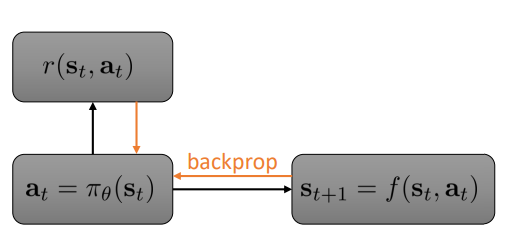
\includegraphics[width=0.49\textwidth]{images/Backprop.PNG}
  %  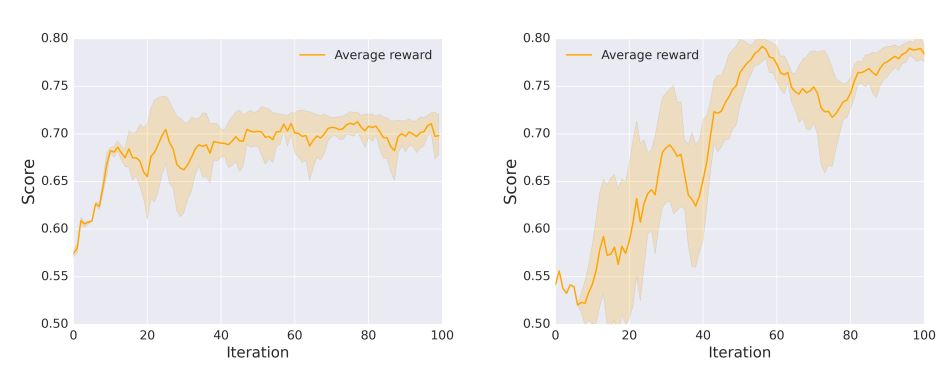
\includegraphics[width=0.49\textwidth]{images/reward_value.JPG}
      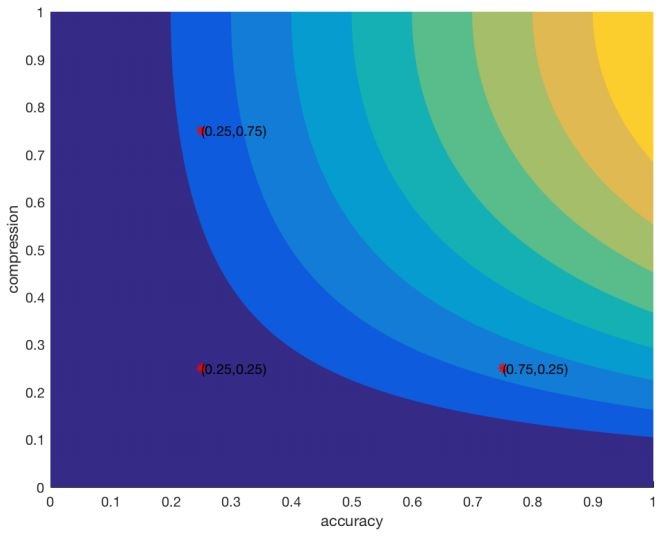
\includegraphics[width=0.49\textwidth]{images/reward_manifold.JPG}
\caption{Reward update strategy with back-propagation and reward manifold}
    \label{fig:moq}
  \end{figure}

  \begin{figure*} 
    \centering
%    \includegraphics[width=0.89\textwidth]{images/L.PNG}
\caption{Learning the value of information and reward over time. Model predictions. (a) In the unequal information condition (when information concerning the packet is not always available), sRL (right frames) predicts a higher probability of choosing highly rewarded option (i.e., exploitation), whereas kRL (left frames) predicts a higher probability of choosing the most informative/never experienced option (i.e., 0seen).  }
    \label{fig:value}
  \end{figure*}

In our experiments described below, we used several approaches for selecting the conditional plan $\pi$:
%\begin{enumerate}
%\item {Random sampling, observation times are selected
%uniformly at random, leading to time intervals of random length independent of the current activity. At time 1, a sample was guaranteed to be made.}

%\item{ Entropy based method acquires data according to a conditional plan π as to minimize the uncertainty in the marginal probability distributions $P(A_t = a | \pi(a))$, measured using the entropy criterion. This strategy
%directly aims at improving the classification accuracy
%of the different activities by solving the optimization problem
%\begin{equation}
%H(A_t | \pi(a)) = -\sum\limits_{x} P(A_t =x | \pi(a)) log %P(A_t = x | \pi(a))
%\end{equation}} \end{enumerate}


Random sampling strategies results in
different sampling points even for the same data. To get a representative result, the means from 30 random trials are shown. Entropy-based strategy was deterministic, thus only one trial is shown.

\subsection{ Sensor Settings Management}
The raw data from the inertial sensor is utilized to examine the power efficiency achieved under different sampling and duty cycling strategies. 

\begin{algorithm}[h]\label{algorithm}
\KwIn{ Taining dataset $X = \{x_1, x_2, ..., x_m\}$, Number of layers $L$}


\KwOut{Class labels}
    {\caption{\bf Dynamic Adaptation Algorithm} \label{Algorithm1}
    }
\end{algorithm}




\subsection{Discrete Action Space}

%https://ieeexplore.ieee.org/stamp/stamp.jsp?tp=&arnumber=7471433
 \begin{figure}
    \centering
    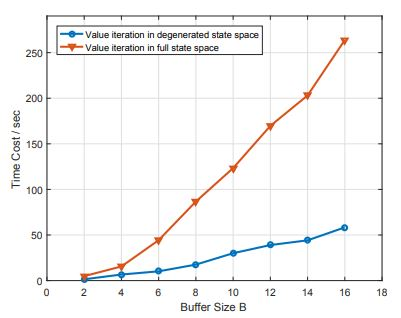
\includegraphics[width=0.39\textwidth]{images/Valueiteration.jpg}
\caption{ Value iteration in degenerated and full state space}
    \label{fig:action}
  \end{figure}
 
  \begin{figure*}
    \centering
    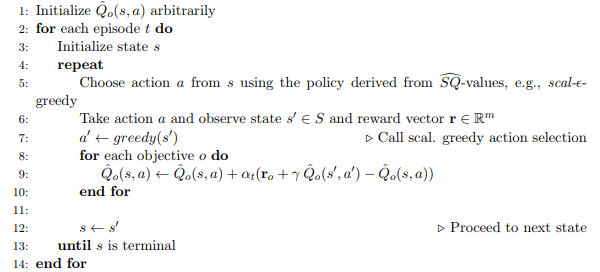
\includegraphics[width=0.69\textwidth]{images/Multi-objectiveQ-learning.PNG}
\caption{Multi-objective Q-learning strategy for updating action space}
    \label{fig:moq}
  \end{figure*}
  
  \subsection{Action bias mean}
 
 %%%%%%%%%%%%%%%%%% RESULTS %%%%%%%%%%%%%%%%%%
\section{RESULTS AND DISCUSSION} \label{sec:results}

 
  
  \subsection{Activity recognition accuracy using different Sampling frequency}
  We report on the energy overheads and the classification accuracy for different combinations of sampling frequency (SF).
  





 

  \begin{figure}
    \centering
    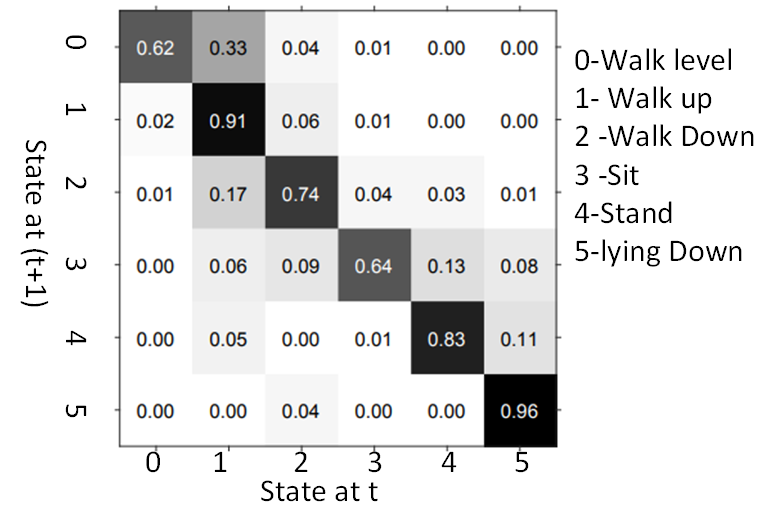
\includegraphics[width=0.39\textwidth]{images/MDP_Confusion.png}
%   \includegraphics[width=0.49\textwidth]{images/FP_FN_detection_change.PNG}
% \caption{False positives (FP) versus false negatives (FN).}

\caption{Transition probabilities between user activity states at t and t+1}
    \label{fig:accuracy}
  \end{figure}
  
  
  \begin{figure}
    \centering
%    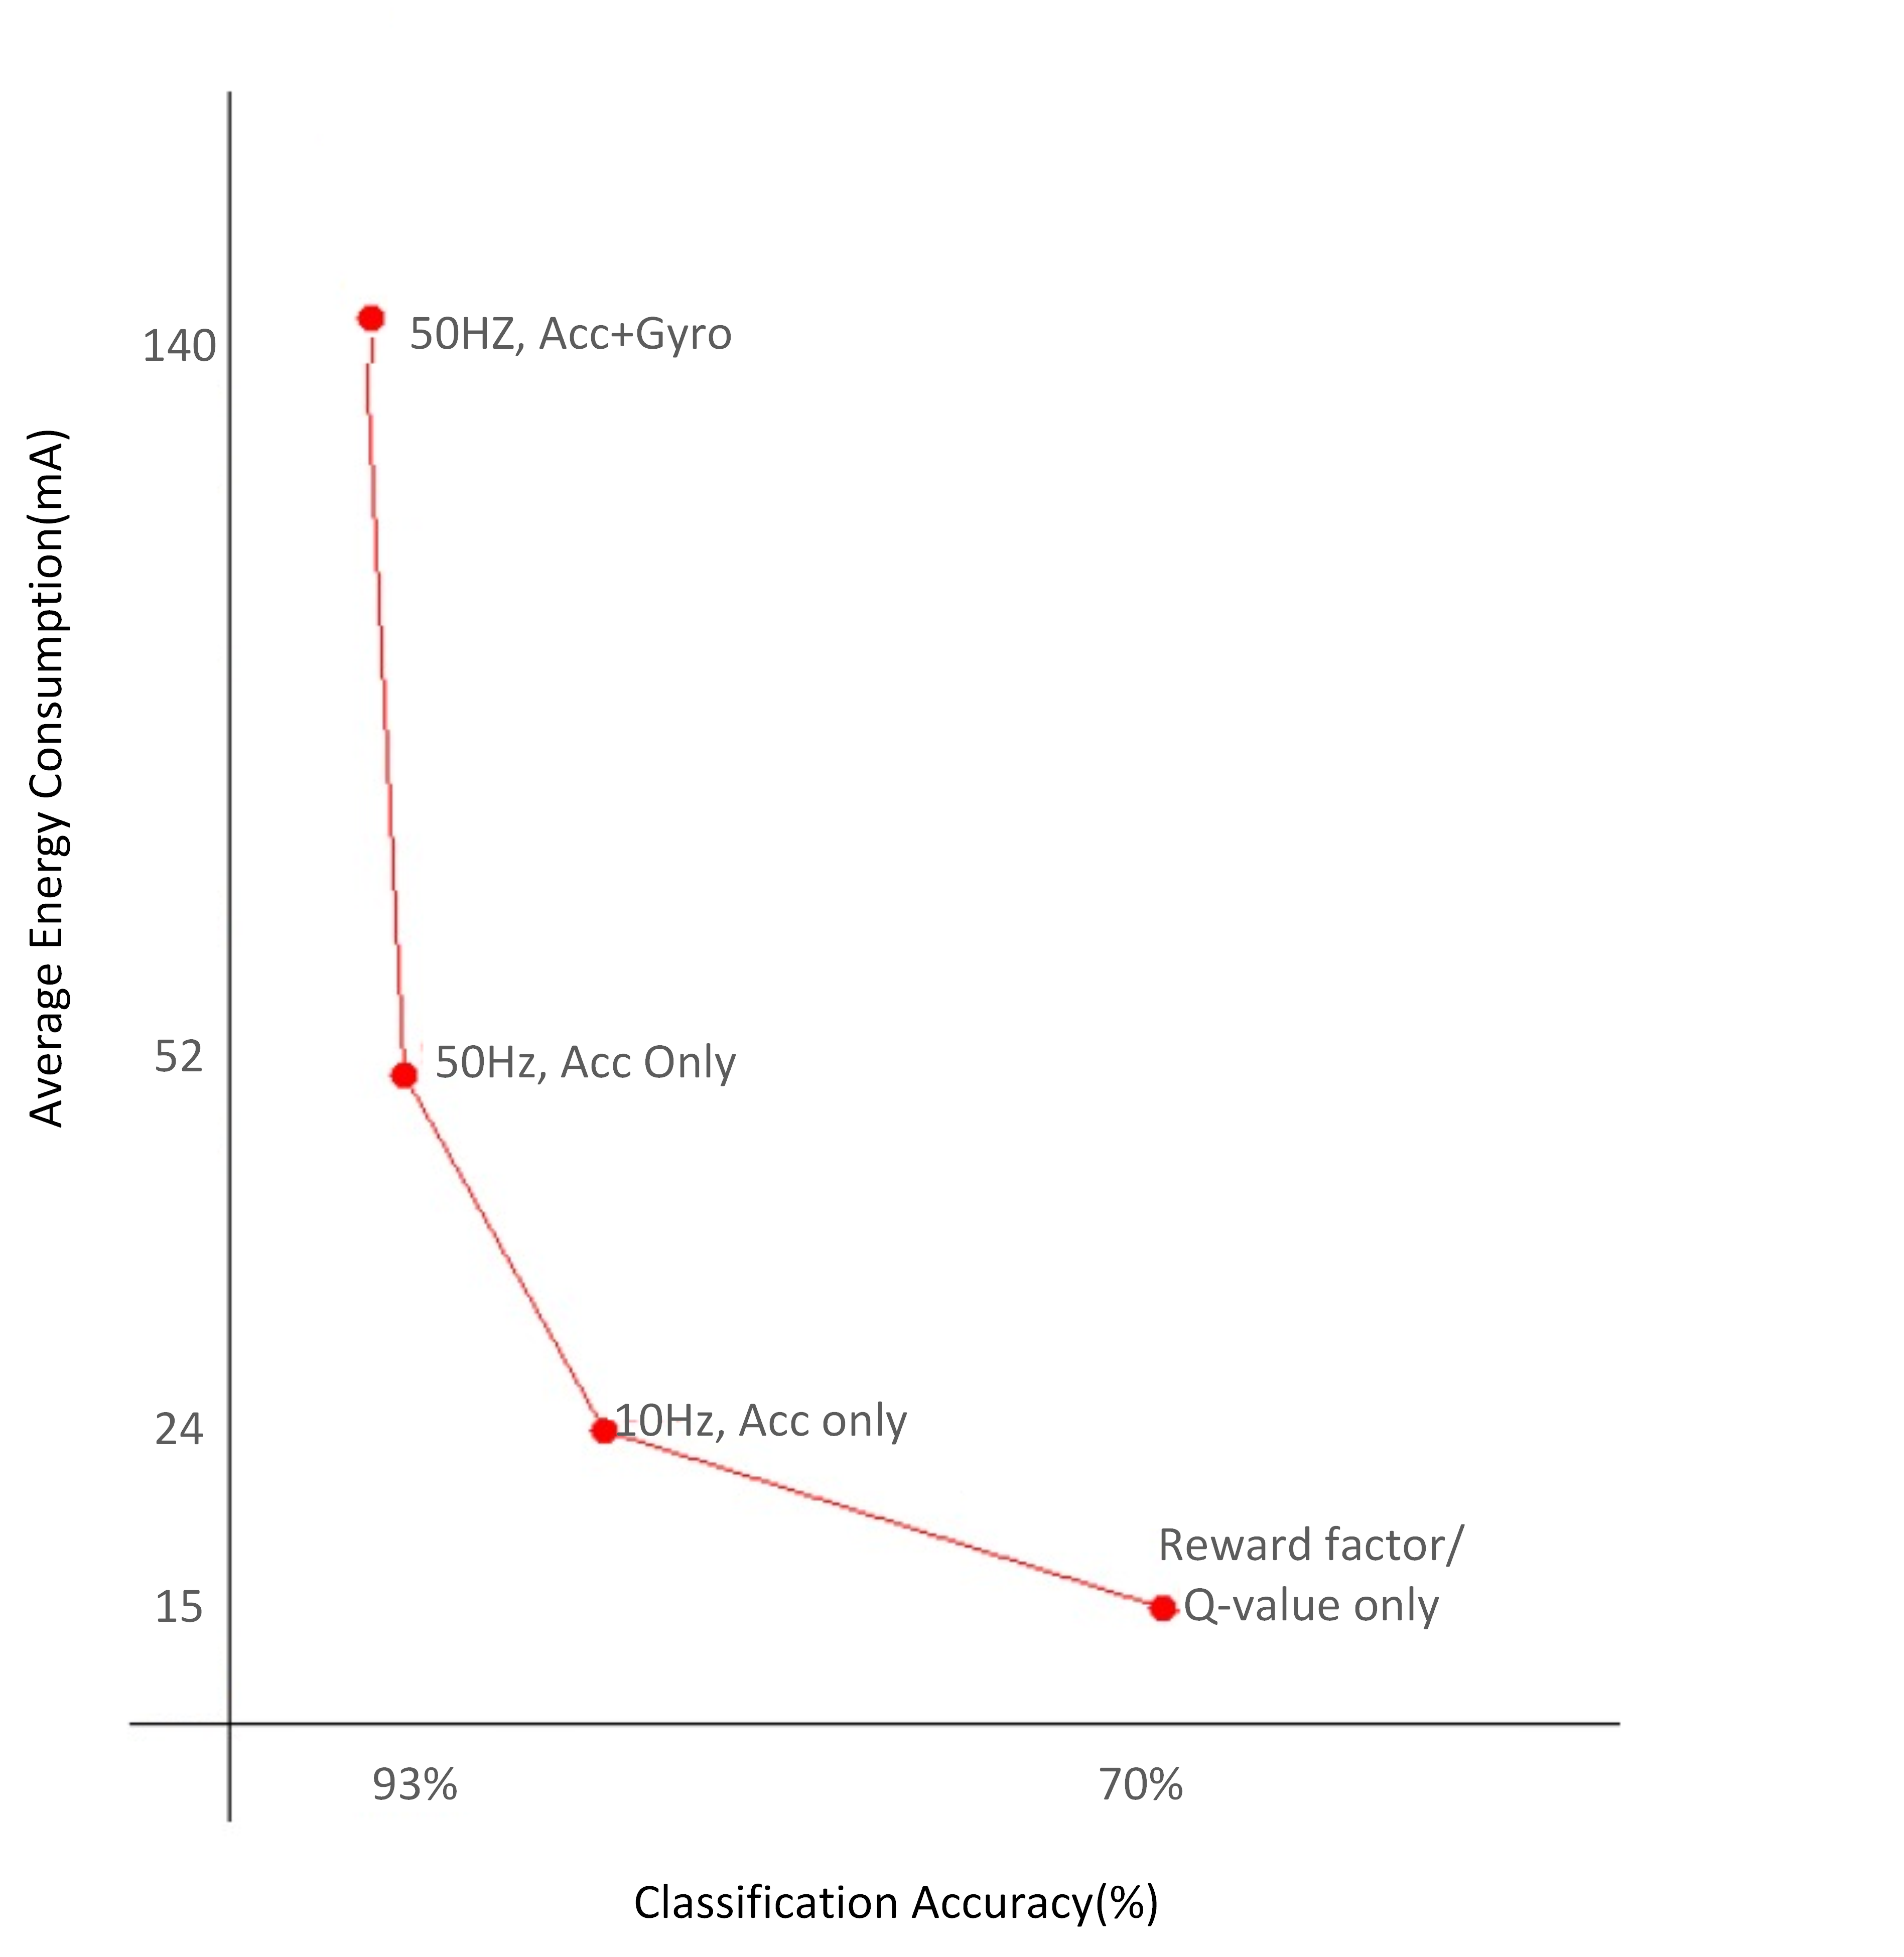
\includegraphics[width=0.49\textwidth]{images/MDP_RESULT.png}
\caption{Energy saving can be achieved by using a converged Q-table for action selection}
    \label{fig:res1}
  \end{figure}
  
  
  \begin{figure}
    \centering
%    \includegraphics[width=0.49\textwidth]{images/MDP_RESULT2.png}
\caption{Action Space selection policy on sensor test frames}
    \label{fig:res2}
  \end{figure}

  

\subsection{Compressed Predictive States}
We finally output a look up table as a special case of a the linear function approximation of the state to action mapping.

\subsection{Comparison with other approaches}

% \begin{equation}
% \phi^{ID}(\mathrm{x})=\phi^{SE}(\mathrm{x})\times\left(\frac{1}{\vert X_{U}\vert}\sum\limits_{\mathrm{x}_{u}\in X_{U}}sim(\mathrm{x},\ \mathrm{x}_{u})\right)^{\beta}
% \tag{1}
% \end{equation}

% Here, the informativeness of x is weighted by its average similarity to all other instances in the unlabeled set  $X_U$ , subject to a parameter  $\beta$  that controls the relative importance of the density term. In the formulation presented above, sequence entropy  $\phi^{SE}$  measures the base informativeness. 

% likelihood function $P(X_{1}^{N})=\sum_{Z_{1}^{N}}P(X_{1}^{N},Z_{1}^{N})=\sum_{i}\alpha(N,s_{i})$

% $P(X_{1}^{N})=\sum_{i}\alpha(N,s_{i})=\alpha(N+1,stop)$

% $\Pi(s)=P(z_{1}=s)=P(s|start)$

% $Q(\theta,\theta^{old})=$ likelihood approximation given $\theta^{old}$

%%%%%%%%%%%%%%%%%% CONCLUSIONS %%%%%%%%%%%%%%%%%%
\section{CONCLUSIONS} \label{sec:conclusions}

We presented a design methodology to
evaluate energy-accuracy trade-offs for querying sensor data from wearable sensors.
We use the framework of Markov Decision Processes
(MDP) to control the sampling rate at the wearable sensor. If we equip an wearable sensor with an MDP
controller, it will regulate the sensing frequency by adapting to the change in the data being measured. the
system as an input.  The main advantage of the MDP controller is that its policy can be computed offline. Only the policy table needs to be stored in the wearable sensor. The operation simply corresponds to looking up the appropriate pre-calculated action (transmit, drop and variable sampling rate) from the policy table. Thus, the operation of this controller places a minimal computational load
on the sensors memory.


Based on the context
history,the results show that the dynamic adaptation
scheme performs better in terms of accuracy
%http://adp.princeton.edu/Papers/Powell_ADP_2ndEdition_Chapter%206.pdf
\FloatBarrier 

%%%%%%%%%%%%%%%%%% REFERENCES %%%%%%%%%%%%%%%%%%
\renewcommand*{\bibfont}{\small}

\printbibliography
 

\end{document}
